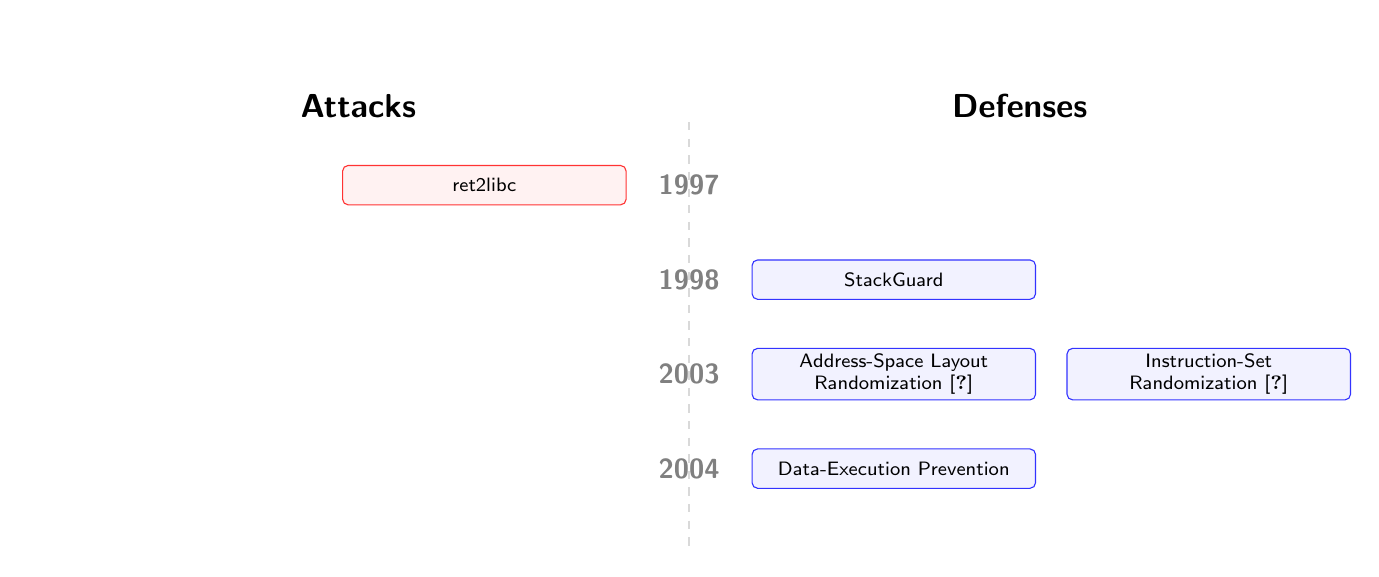
\begin{tikzpicture}[year node/.style={font=\bfseries\sffamily\color{gray}, align=center, inner sep=2pt},attack node/.style={draw=red!80, fill=red!5, rounded corners=2pt, font=\scriptsize\sffamily, align=center, minimum width=3.60cm, minimum height=0.5cm, inner sep=2pt, text width=3.40cm, execute at begin node=\setlength{\emergencystretch}{0pt}\tolerance 200\hyphenpenalty 10000\exhyphenpenalty 10000},defense node/.style={draw=blue!80, fill=blue!5, rounded corners=2pt, font=\scriptsize\sffamily, align=center, minimum width=3.60cm, minimum height=0.5cm, inner sep=2pt, text width=3.40cm, execute at begin node=\setlength{\emergencystretch}{0pt}\tolerance 200\hyphenpenalty 10000\exhyphenpenalty 10000},spine/.style={thick, gray!30, dashed}]%
\node[font=\large\bfseries\sffamily] at (-4.2,1.0) {Attacks};%
\node[font=\large\bfseries\sffamily] at (4.2,1.0) {Defenses};%
  % Year 1997%
\node[year node] at (0.0,0.0) {1997};%
\node[attack node] at (-2.6,0.0) {ret2libc};%
  % Year 1998%
\node[year node] at (0.0,-1.2) {1998};%
\node[defense node] at (2.6,-1.2) {StackGuard};%
  % Year 2003%
\node[year node] at (0.0,-2.4) {2003};%
\node[defense node] at (2.6,-2.4) {Address{-}Space Layout\\ Randomization \allowbreak\cite{PaXTeam2003}};%
\node[defense node] at (6.6,-2.4) {Instruction{-}Set\\ Randomization \allowbreak\cite{boyd2010}};%
  % Year 2004%
\node[year node] at (0.0,-3.6) {2004};%
\node[defense node] at (2.6,-3.6) {Data{-}Execution Prevention};%
\path[spine,draw] (0.0,0.8) -- (0.0,-4.6);%
\path[use as bounding box] (-8.40,-4.60) rectangle (8.40,2.00);%
\end{tikzpicture}